\documentclass[tikz,border=5mm]{standalone}
\begin{document}

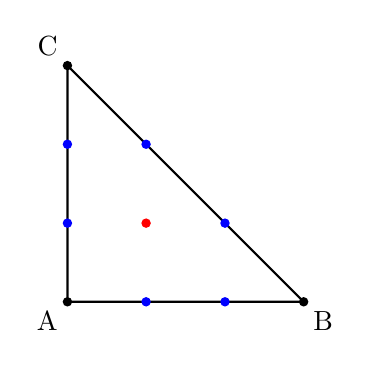
\begin{tikzpicture}[scale=3]

  % Define the vertices of the reference triangle
  \coordinate (A) at (0,0);
  \coordinate (B) at (1,0);
  \coordinate (C) at (0,1);

  % Draw the triangle
  \draw[thick] (A) -- (B) -- (C) -- cycle;

  % Define and draw the order 3 Lagrange nodes
  \coordinate (D) at (0.333,0);
  \coordinate (E) at (0.667,0);
  \coordinate (F) at (0.667,0.333);
  \coordinate (G) at (0.333,0.667);
  
  \coordinate (H) at (0,0.333);
  \coordinate (I) at (0,0.667);
  \coordinate (J) at (0.333,0.333);

  % Vertex nodes
  \fill[black] (A) circle (0.02);
  \fill[black] (B) circle (0.02);
  \fill[black] (C) circle (0.02);

  % Edge nodes
  \fill[blue] (D) circle (0.02);
  \fill[blue] (E) circle (0.02);
  \fill[blue] (H) circle (0.02);
  \fill[blue] (I) circle (0.02);
  \fill[blue] (F) circle (0.02);
  \fill[blue] (G) circle (0.02);

  % Internal node
  \fill[red] (J) circle (0.02);

  % Add labels for clarity
  \node[below left] at (A) {A};
  \node[below right] at (B) {B};
  \node[above left] at (C) {C};

%  \node[below] at (D) {1/3};
%  \node[below] at (E) {2/3};
%  \node[right] at (F) {2/3};
%  \node[left] at (G) {1/3};

%  \node[above left] at (H) {1/3};
%  \node[above left] at (I) {2/3};

% Label the internal node
%  \node at (J) {(1/3, 1/3)};

\end{tikzpicture}

\end{document}

